\section{Results}

\subsection{Level-3 data of chlorophyll-a concentration in the East Sea}

Figure \ref{fig:monLAC01} - \ref{fig:monGAC03}\ are 1 $\rm km$-resolution monthly mean values of chlorophyll-a Level-3 data in the study area which is 34.00$\rm^{\circ}N$ - 44.00$\rm^{\circ}N$, 127.00$\rm^{\circ}E$ - 135.00$\rm^{\circ}E$. The monthly-mean chlorophyll-a concentration of the LAC data from 2003 to 2006 are shown in Figure \ref{fig:monLAC01} - \ref{fig:monLAC03}, and the monthly-mean chlorophyll-a concentration of the GAC data from 2003 to 2006 are shown in Figure \ref{fig:monGAC01} - \ref{fig:monGAC03}. It shows high concentration in Spring (March, April) and fall (October, November).

The black area is part with no data due to cloud coverage or satellite failures. The LAC data in 2005 especially show large black areas because less files had been aggregated compared to other years. The black areas in Winter (January, December) can also been noticed to be larger than other years and this is caused by cloud coverage.

High chlorophyll-a concentration was observed at the sea near Wonsan, Vladivostok, and Pohang. The sea near Wonsan showed high concentration on most of the months, except on May and June. The sea near Vladivostok had high concentrations on spring (March, April) and fall (October, November) when the overall concentration was high. The sea near Pohang showed a chlorophyll-a tail caused by sea current. It occurred quite randomly, and it could be observed well on September to November, 2003. 

Both the LAC and the GAC data showed similar chlorophyll-a distribution, meaning that they are both suitable for sensing spatial and temporal distribution of chlorophyll-a concentration.

\begin{figure}[h]
	\centering
	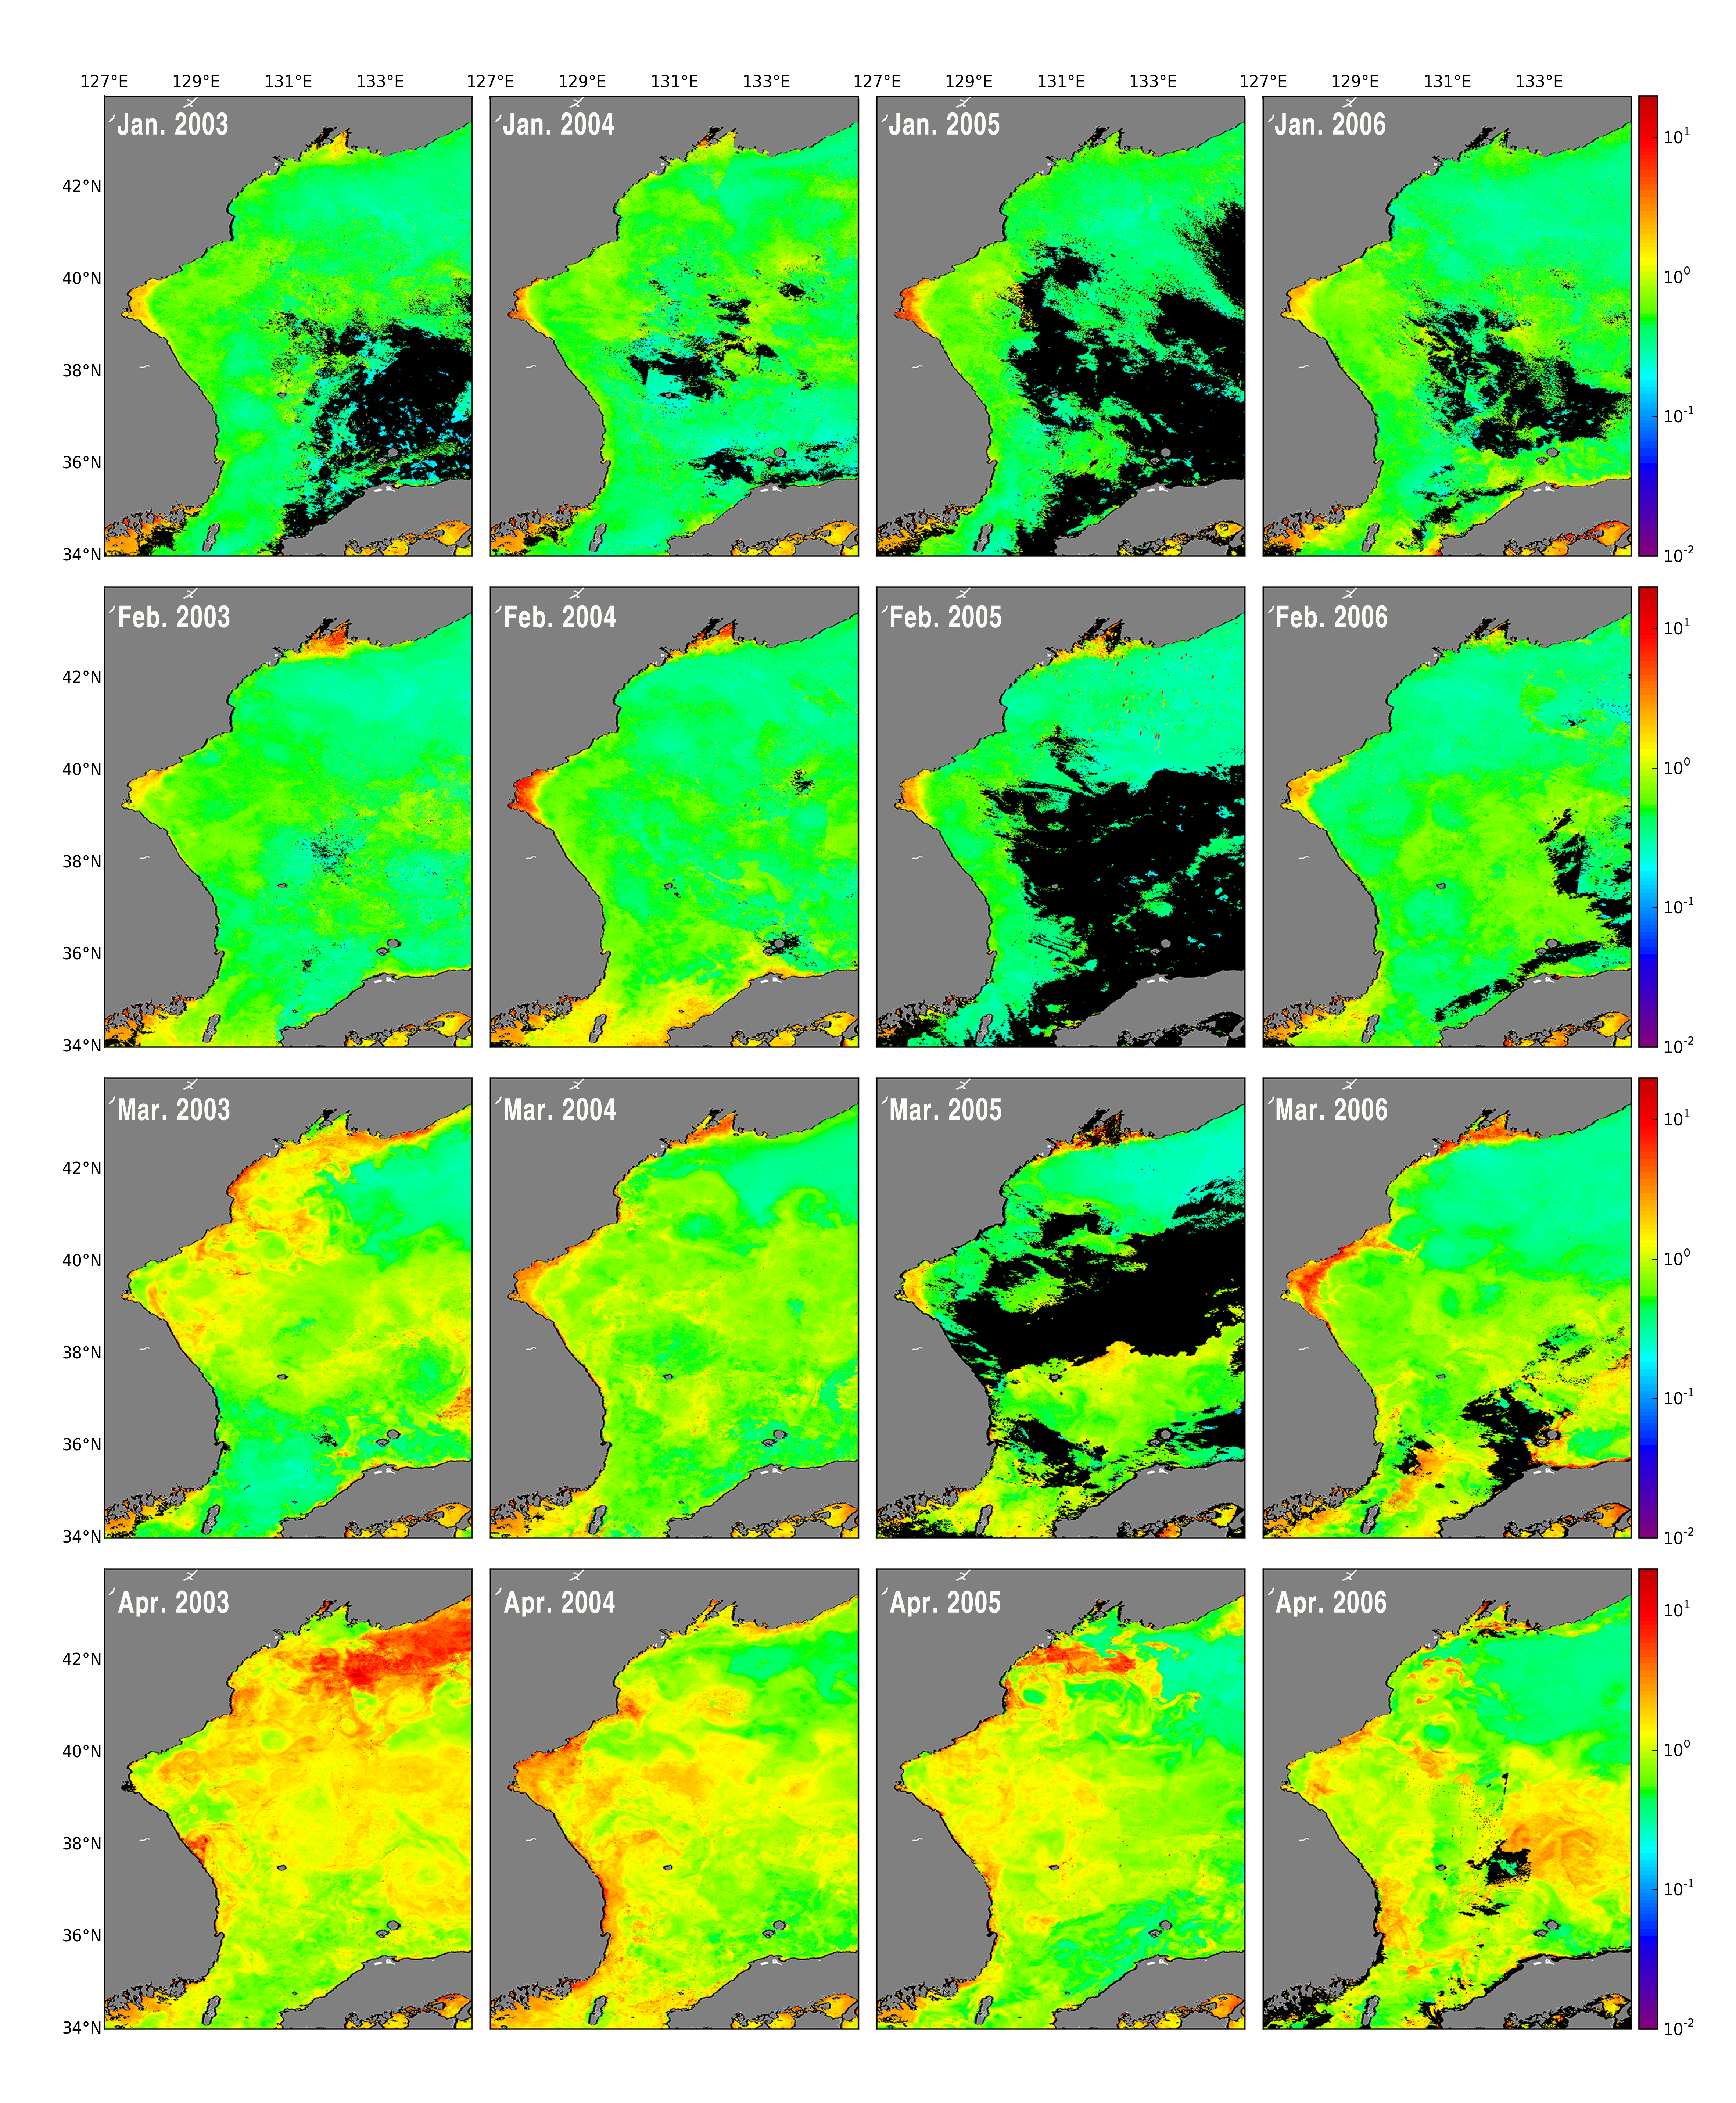
\includegraphics[width=1.0\textwidth]{monLAC01}\\
	\caption{The monthly mean of chlorophyll-a distribution from SeaWiFS LAC data in the East Sea from 2003 to 2006, January to April.}
	\label{fig:monLAC01}
\end{figure}


\begin{figure}[h]
	\centering
	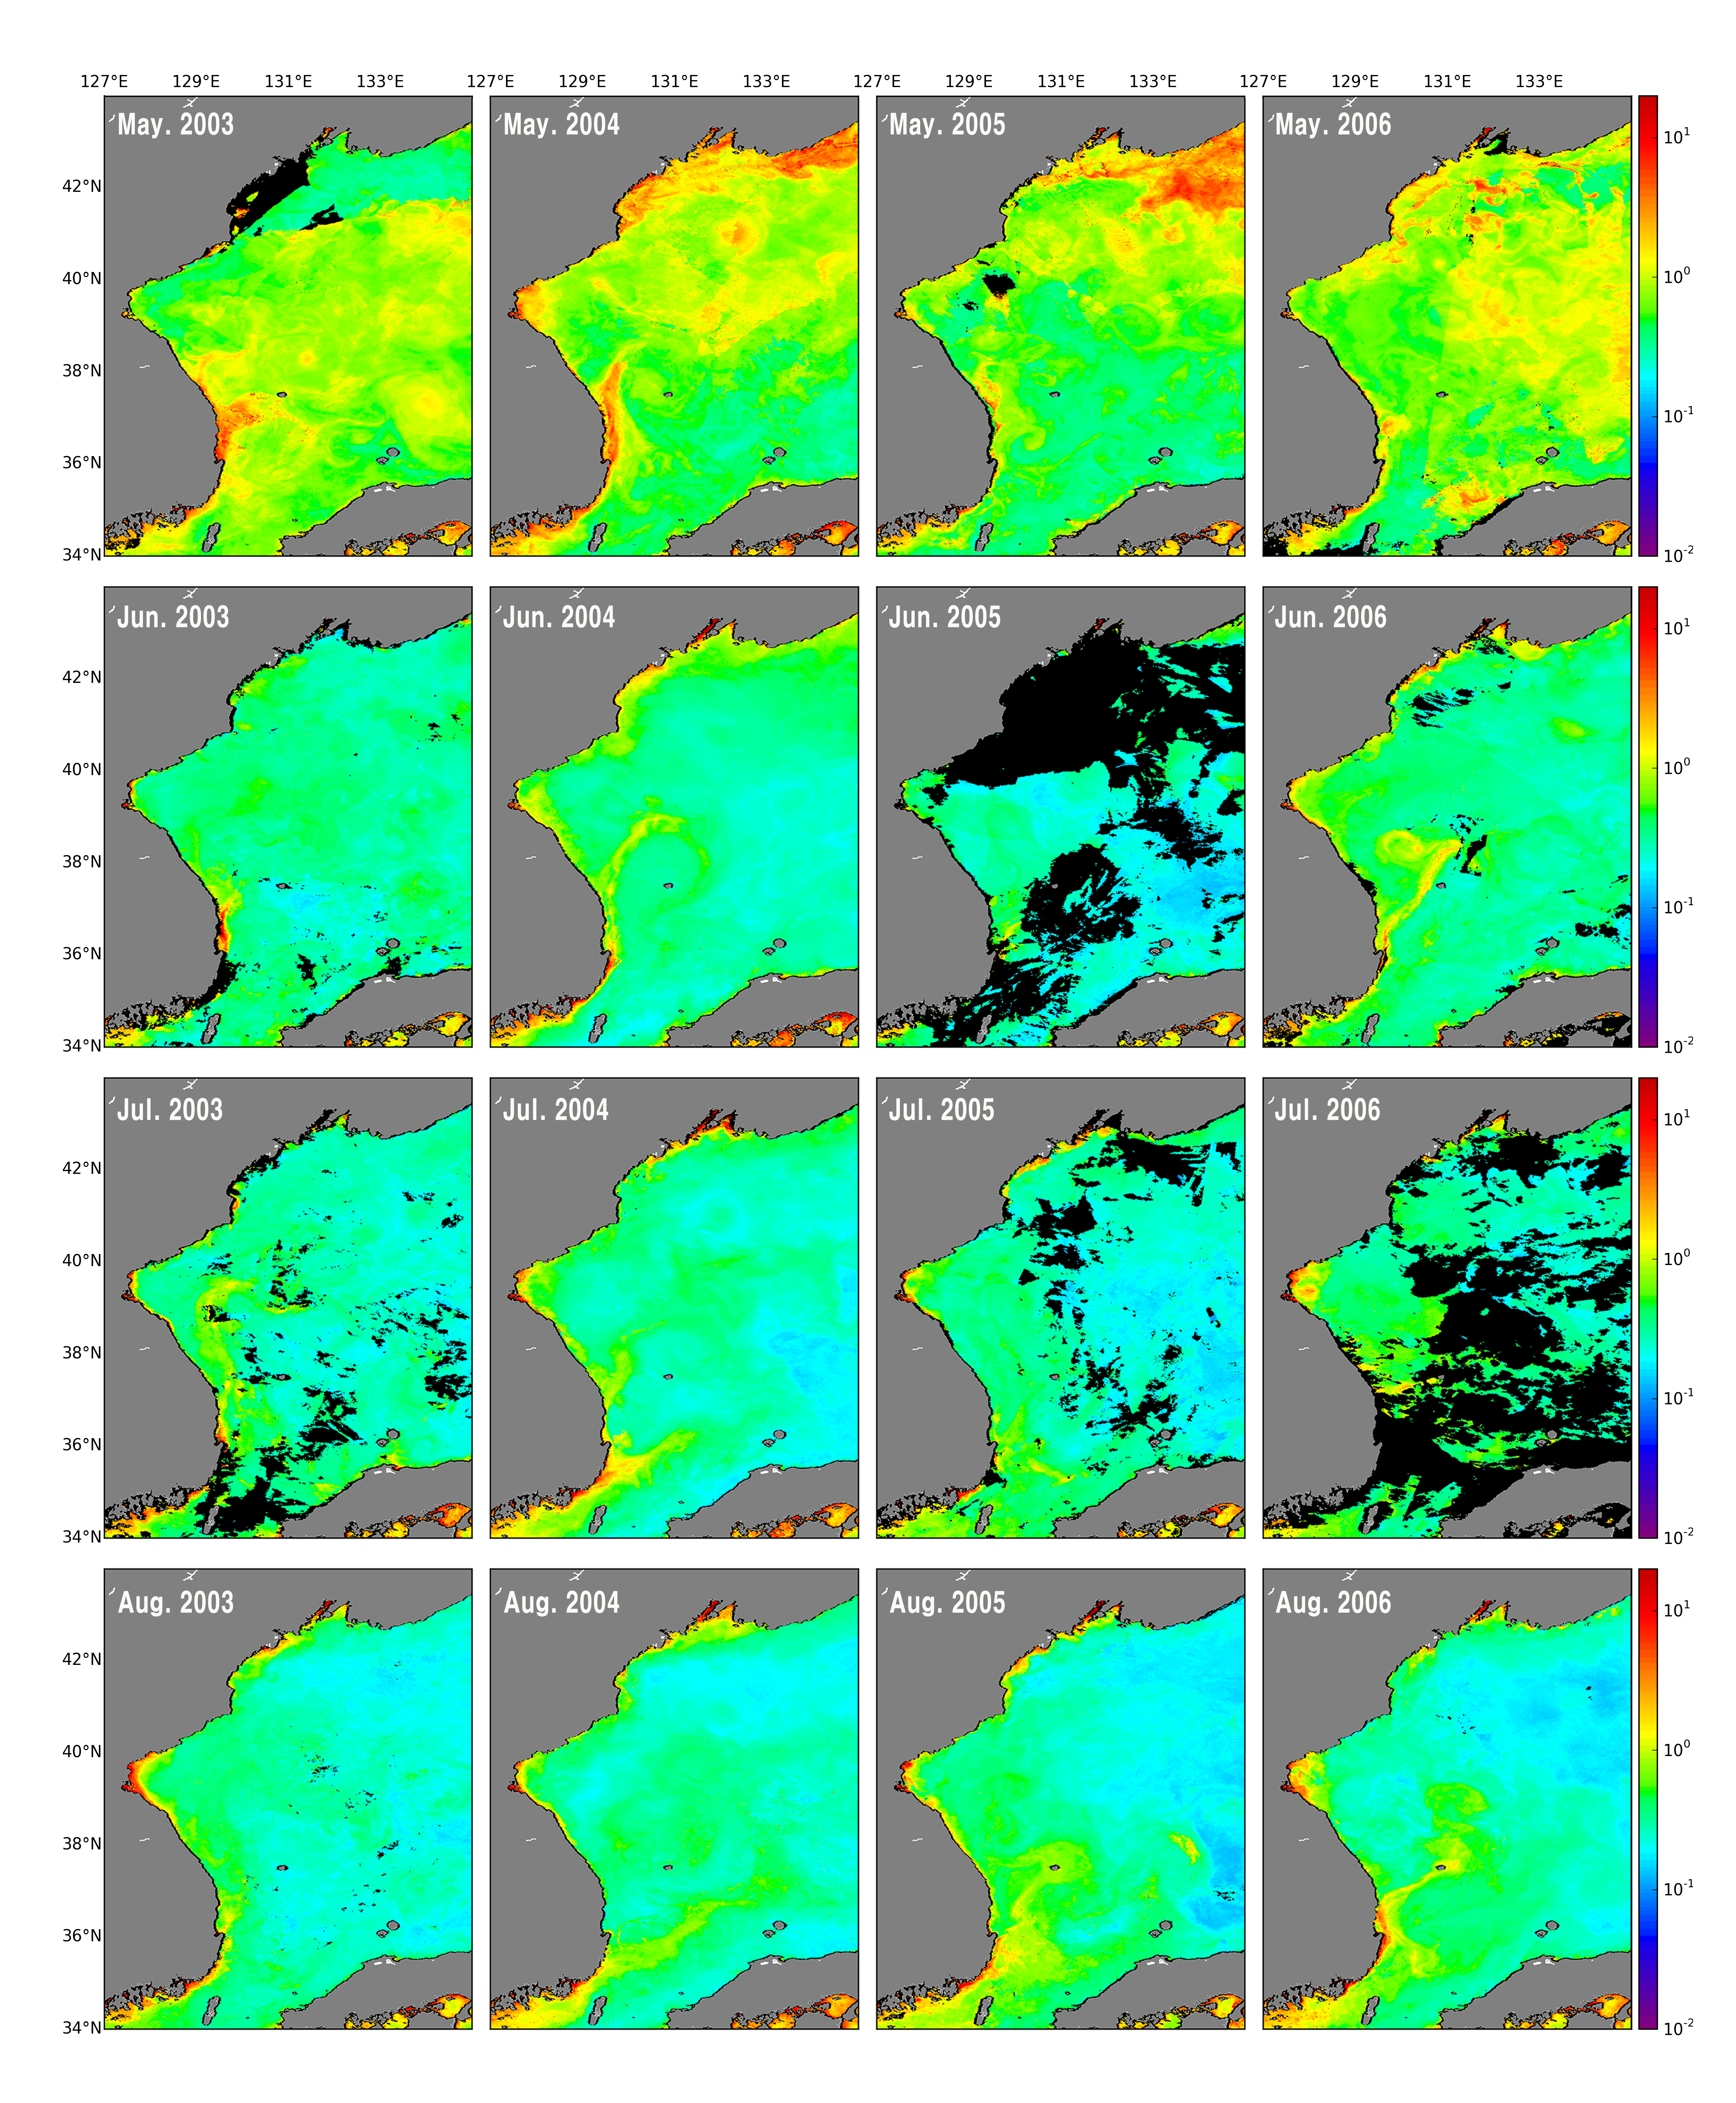
\includegraphics[width=1.00\textwidth]{monLAC02}\\
	\caption{The monthly mean of chlorophyll-a distribution from SeaWiFS LAC data in the East Sea from 2003 to 2006, May to August.}
	\label{fig:monLAC02}
\end{figure}

\begin{figure}[h]
	\centering
	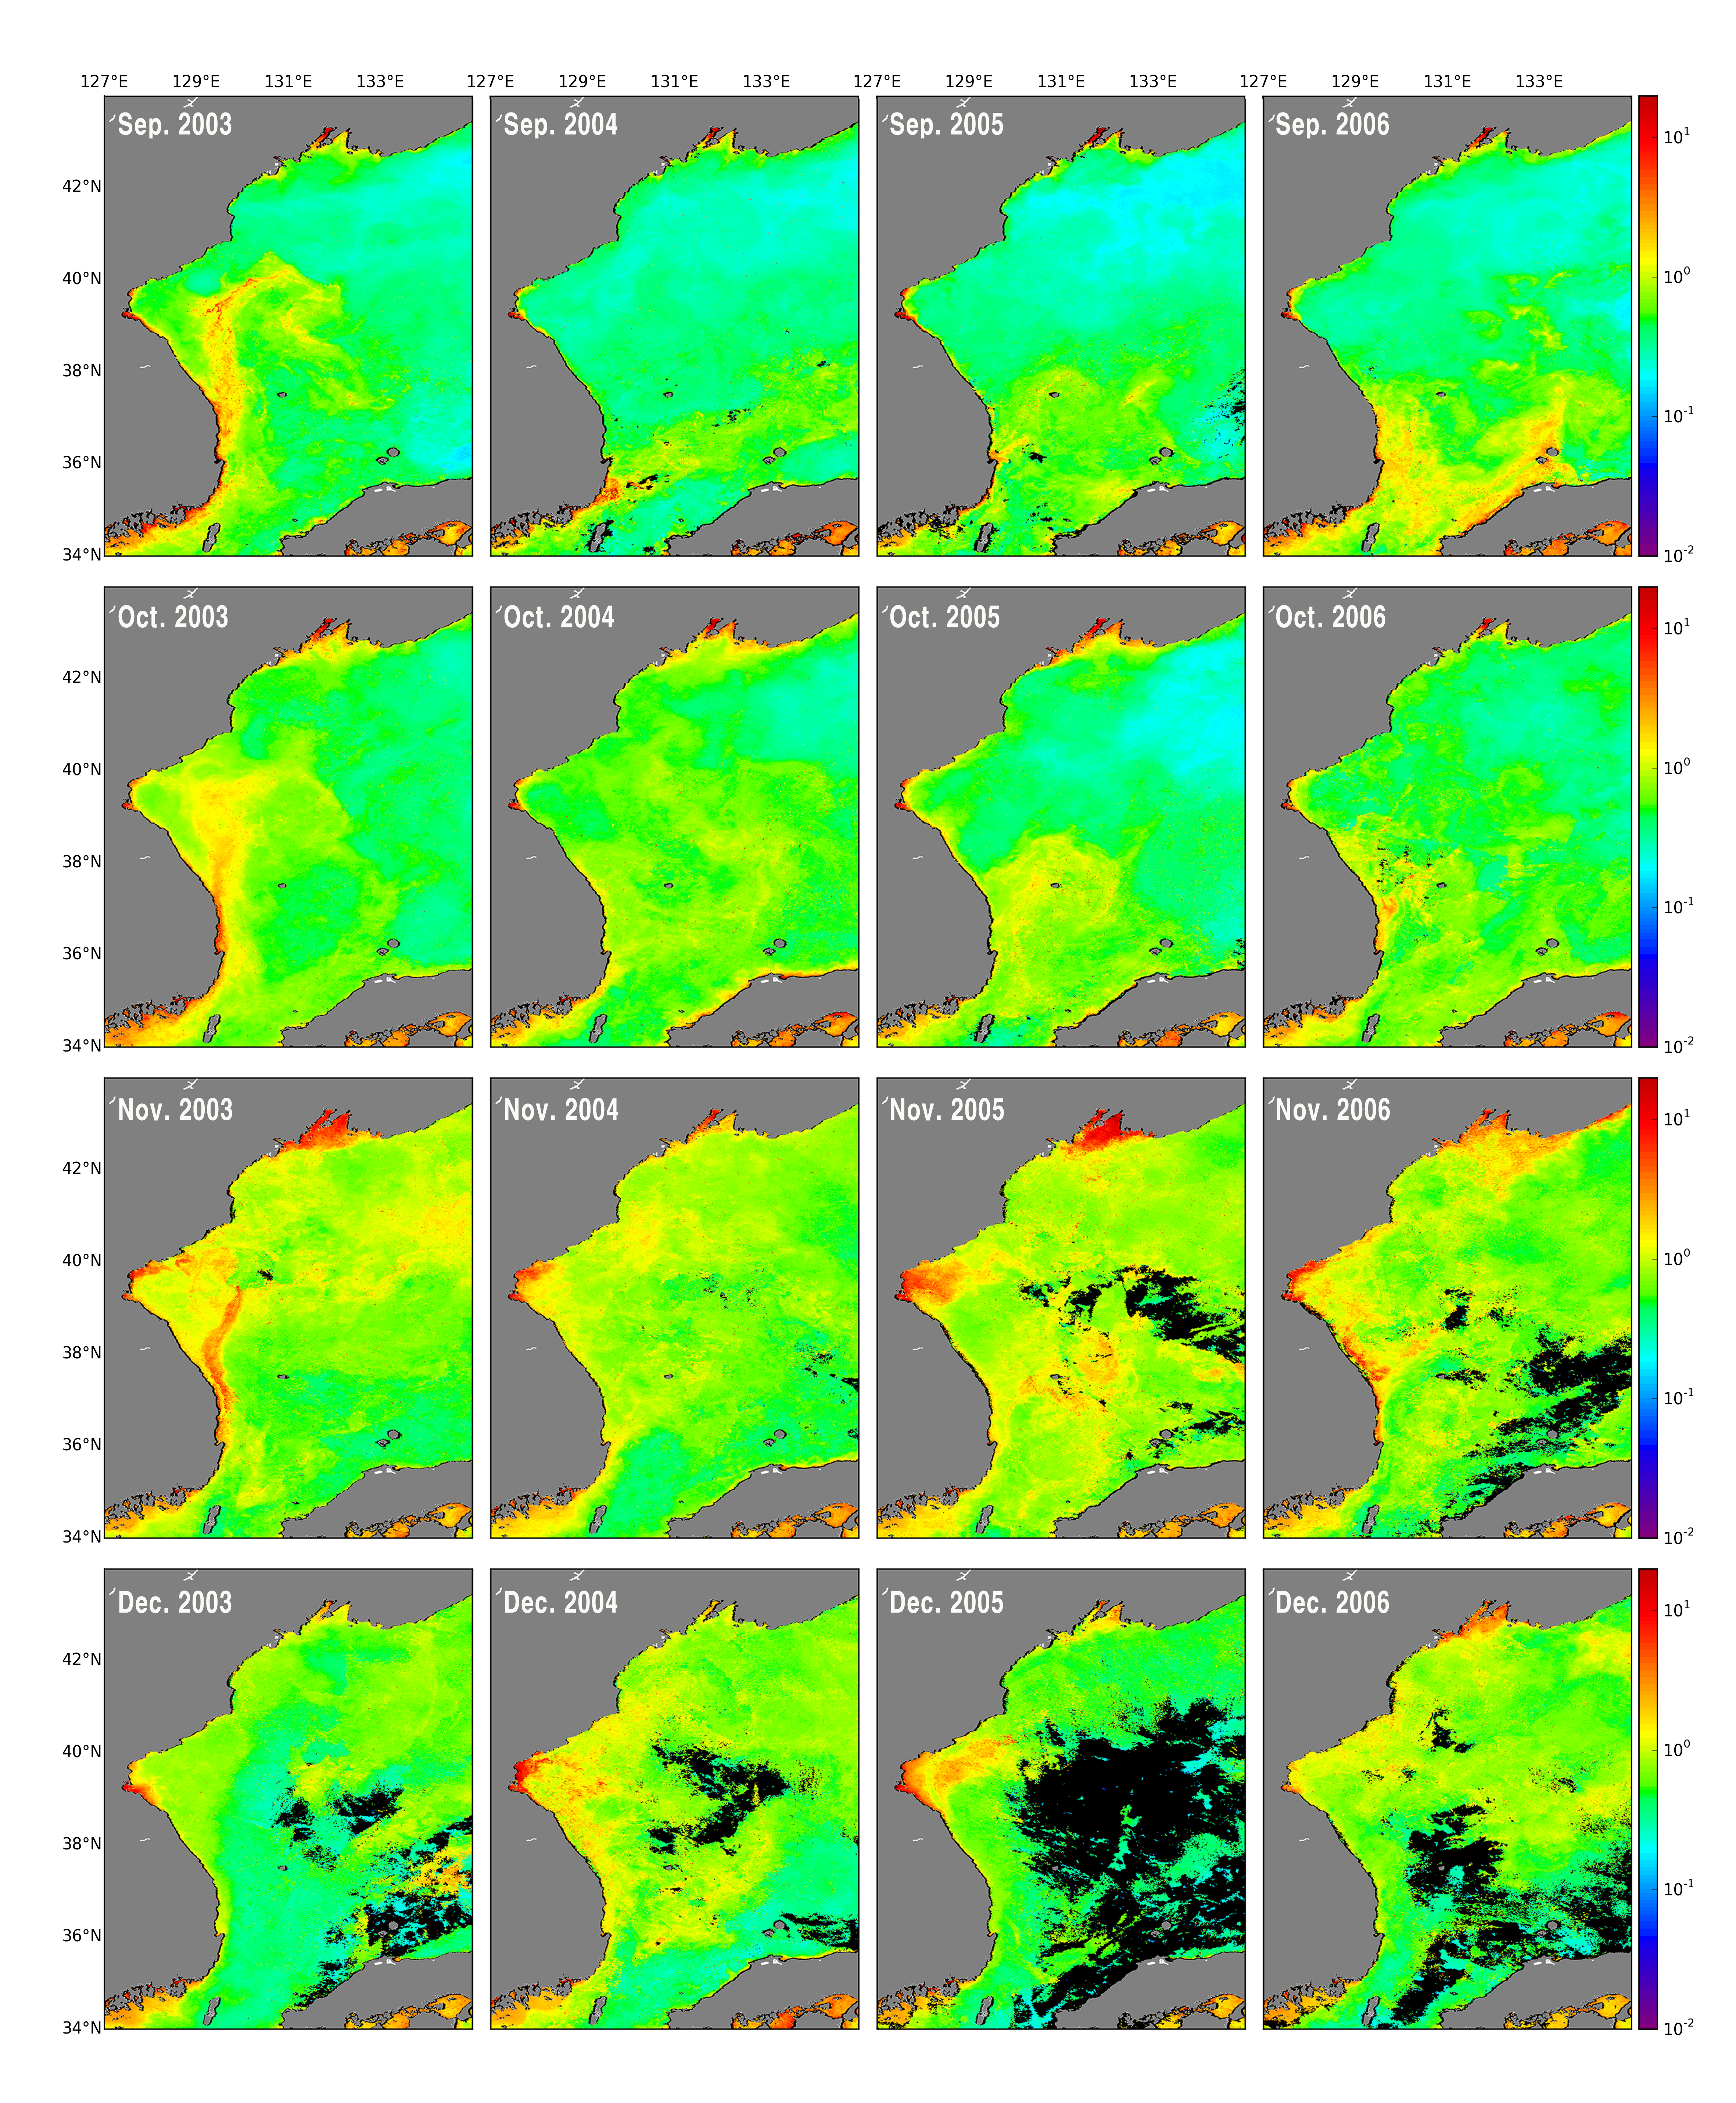
\includegraphics[width=1.00\textwidth]{monLAC03}\\
	\caption{The monthly mean of chlorophyll-a distribution from SeaWiFS LAC data in the East Sea from 2003 to 2006, September to December.}
	\label{fig:monLAC03}
\end{figure}


\begin{figure}[h]
	\centering
	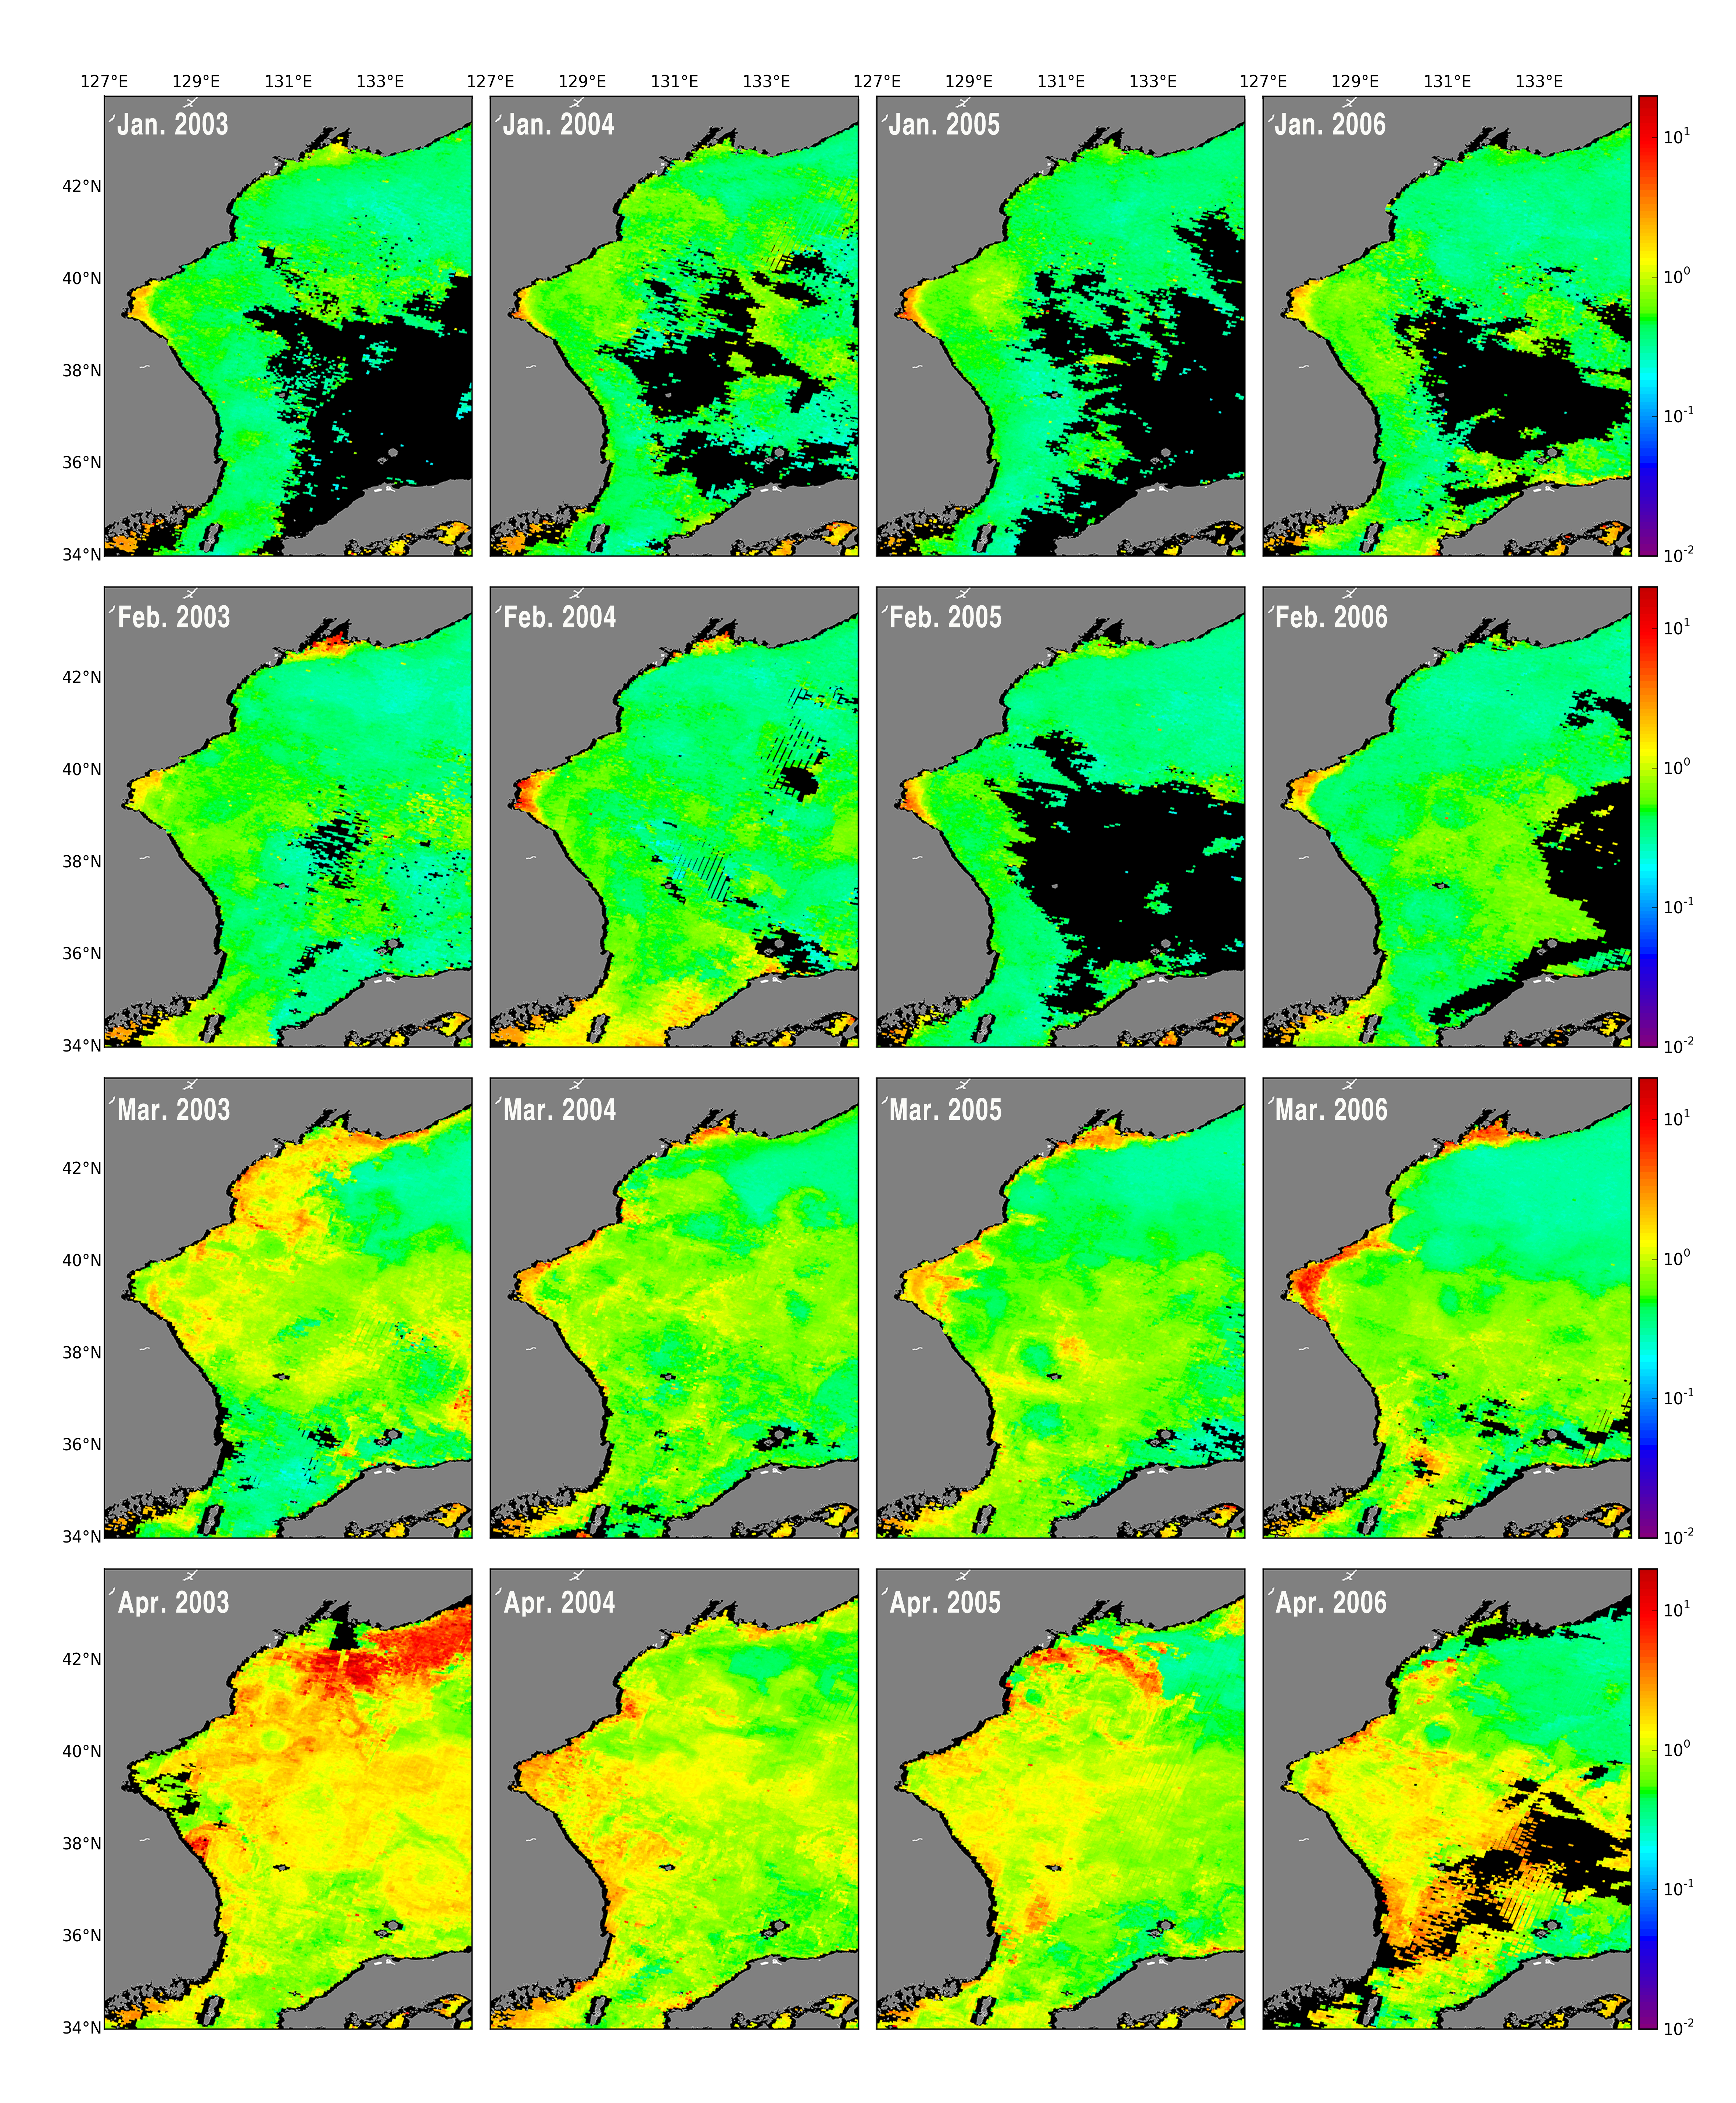
\includegraphics[width=1.0\textwidth]{monGAC01}\\
	\caption{The monthly mean of chlorophyll-a distribution from SeaWiFS GAC data in the East Sea from 2003 to 2006, January to April.}
	\label{fig:monGAC01}
\end{figure}


\begin{figure}[h]
	\centering
	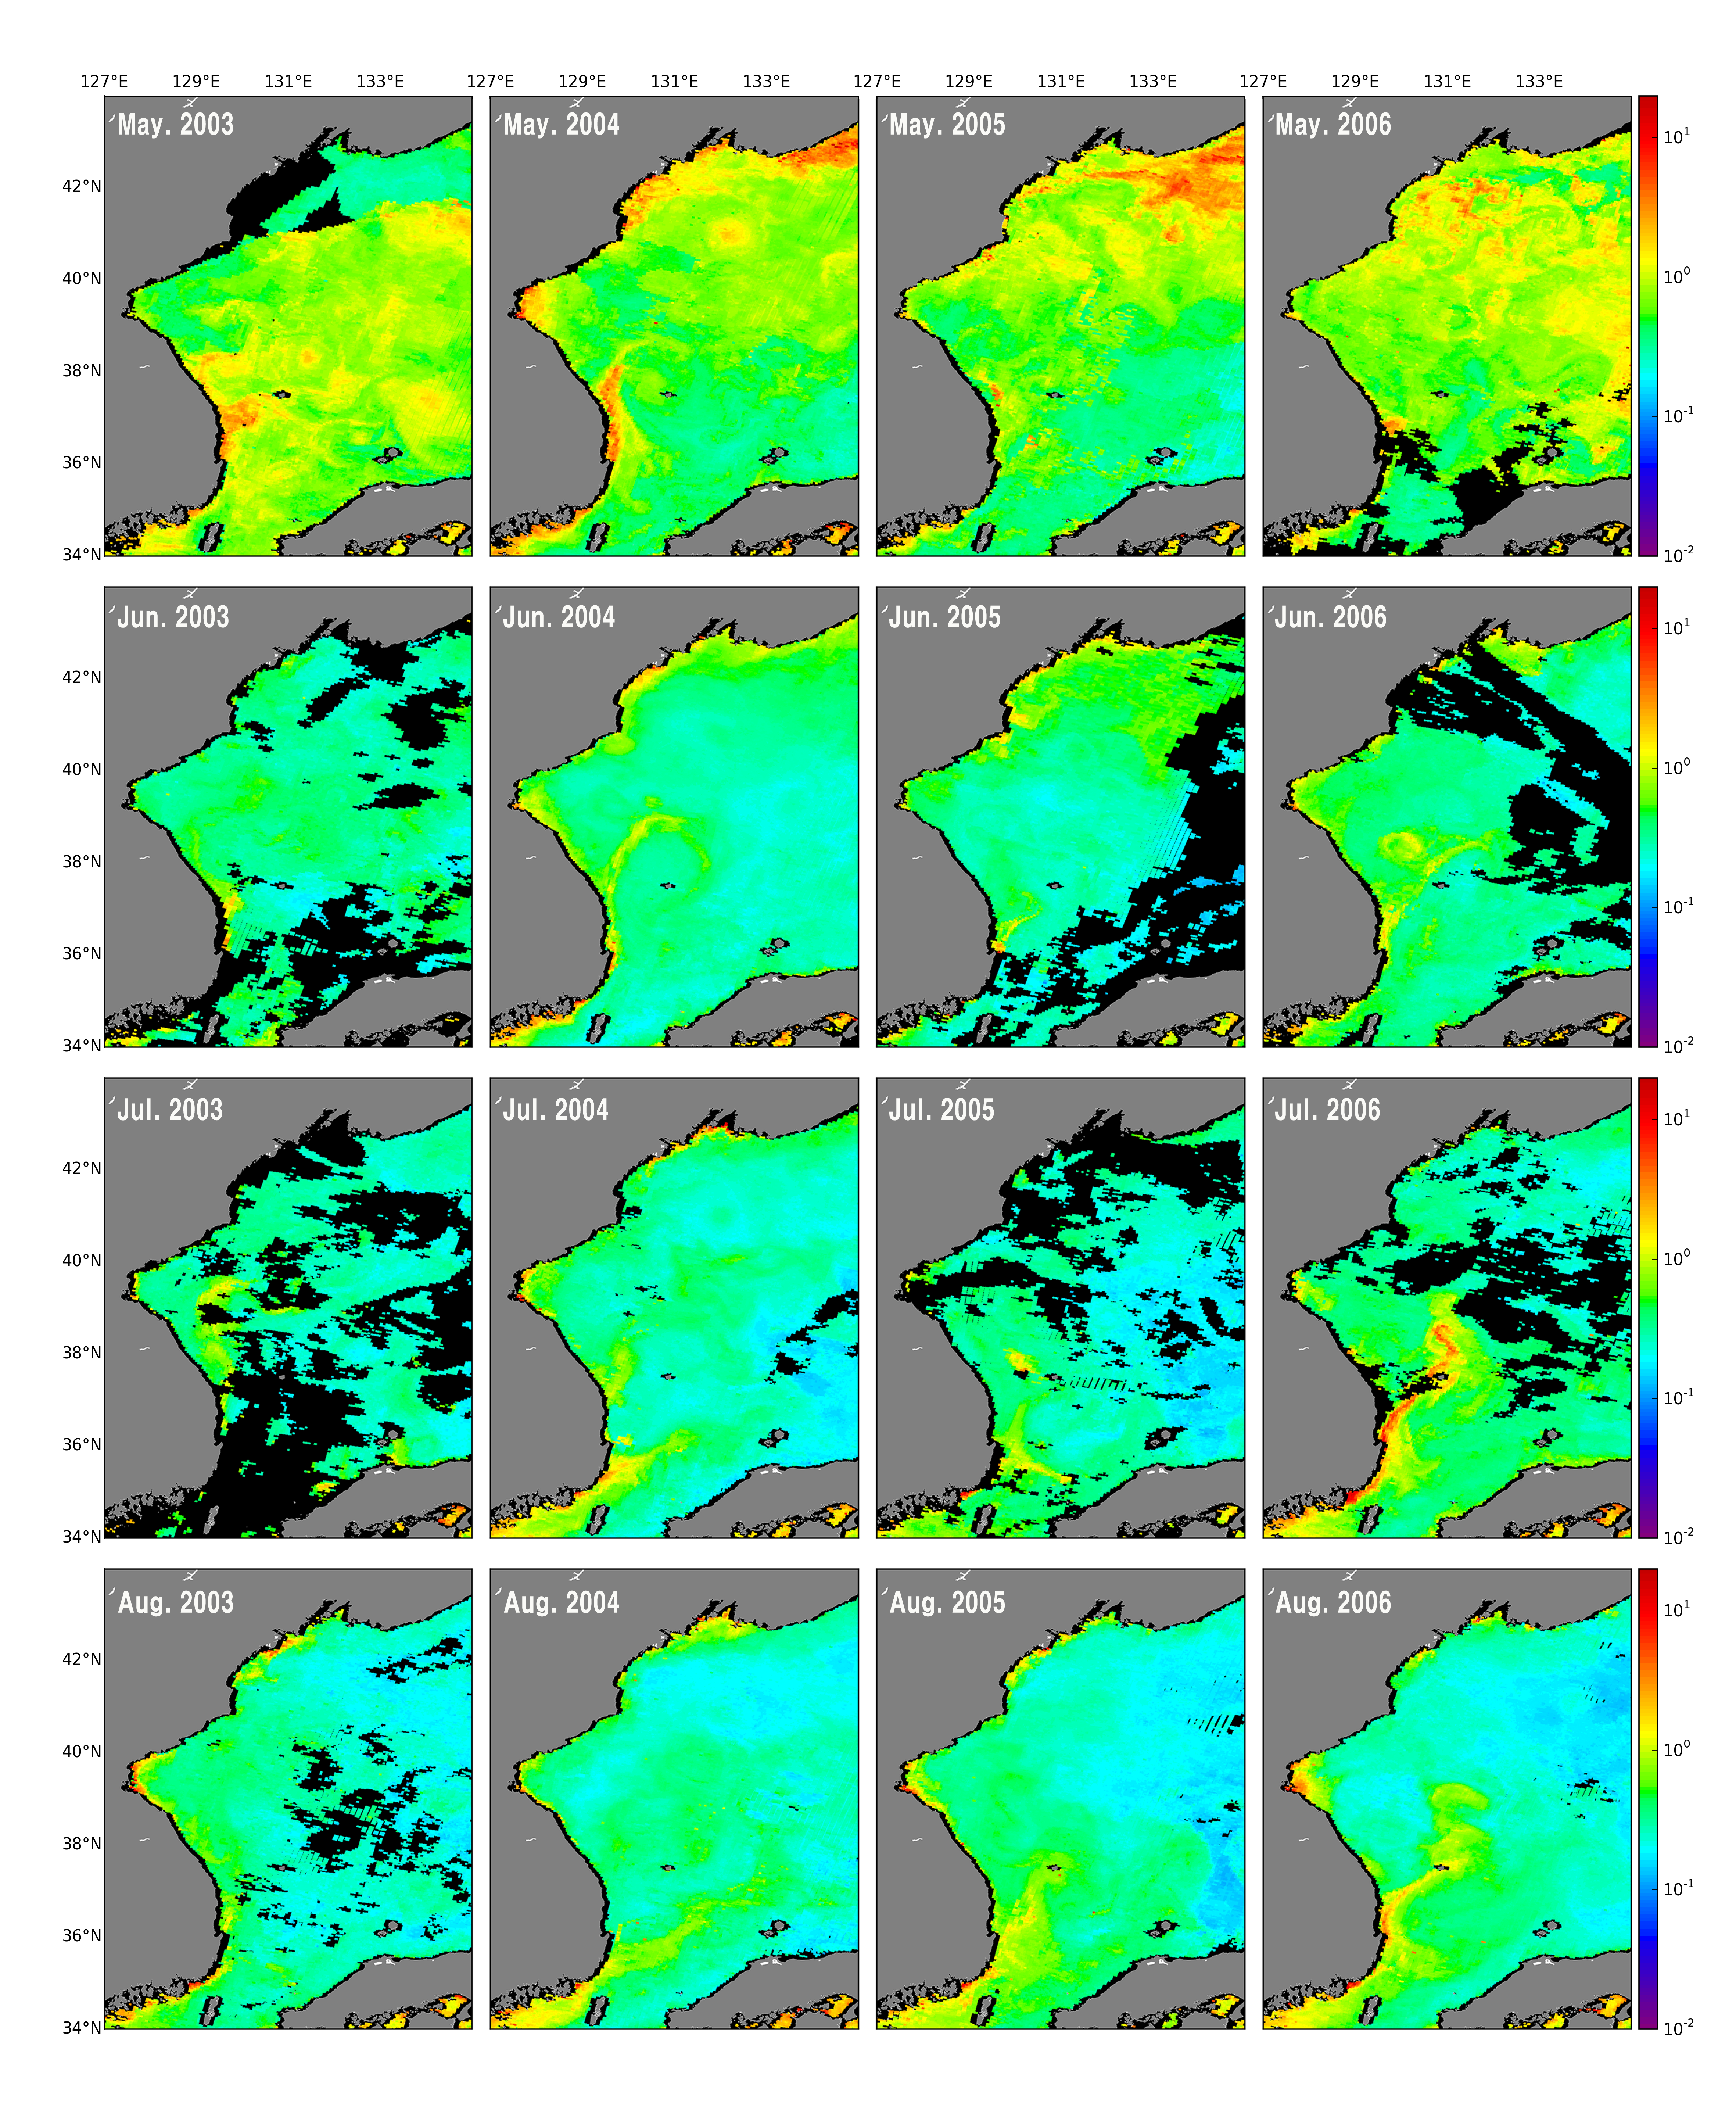
\includegraphics[width=1.00\textwidth]{monGAC02}\\
	\caption{The monthly mean of chlorophyll-a distribution ifrom SeaWiFS GAC data in the East Sea from 2003 to 2006, May to August.}
	\label{fig:monGAC02}
\end{figure}


\begin{figure}[h]
	\centering
	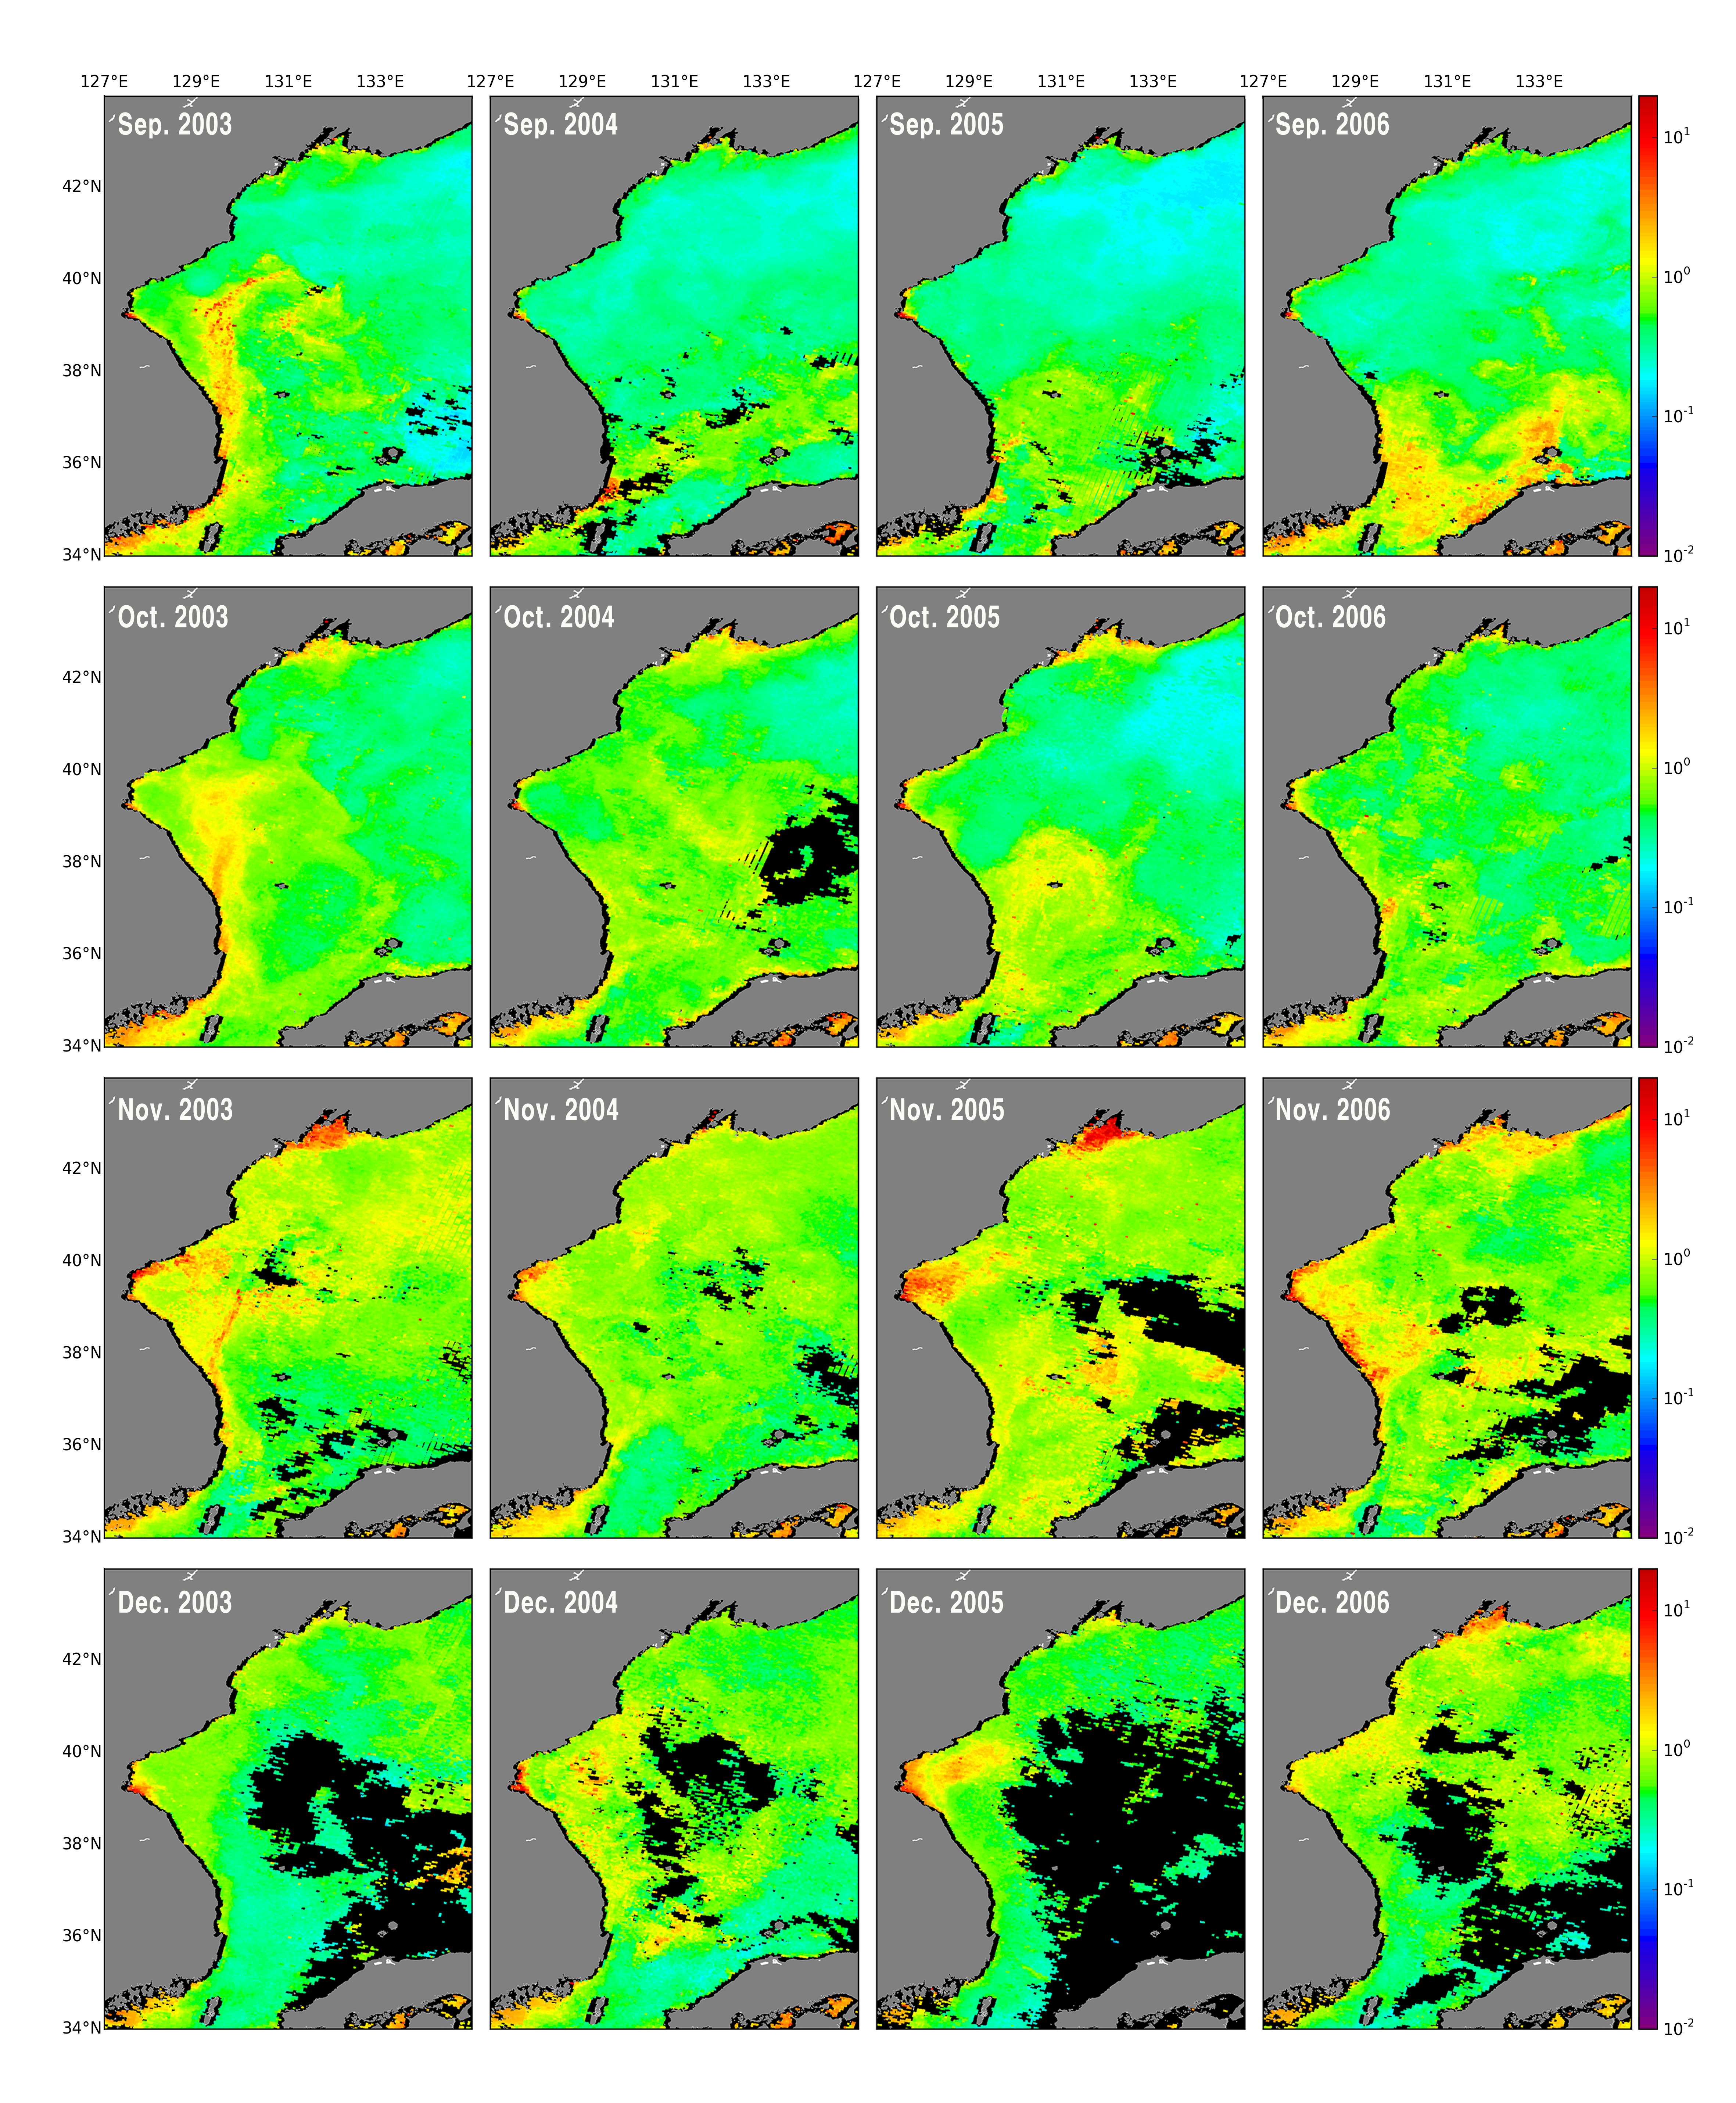
\includegraphics[width=1.00\textwidth]{monGAC03}\\
	\caption{The monthly mean of chlorophyll-a distribution from SeaWiFS LAC data in the East Sea from 2003 to 2006, September to December.}
	\label{fig:monGAC03}
\end{figure}
